\documentclass[a4paper, 12pt]{article}

% Layout
\usepackage{geometry}
\geometry{left=30mm}
\geometry{right=15mm}
\geometry{top=20mm}
\geometry{bottom=20mm}

% Paragraph
\usepackage{indentfirst}
\setlength{\parindent}{0.75cm}
\linespread{1.25}

% Font
\usepackage{fontspec}
\usepackage[english,russian]{babel}
\usepackage{microtype}

% \usepackage{polyglossia}
% \setmainlanguage{russian}
% \setotherlanguage{english}

% \newfontfamily{\cyrillicfont}{Droid Serif}
% \newfontfamily{\cyrillicfontrm}{Droid Serif}
% \newfontfamily{\cyrillicfontsf}{Droid Sans}
% \newfontfamily{\cyrillicfonttt}{DejaVu Sans Mono}

\setmainfont{Droid Serif}
\setromanfont{Droid Serif}
\setsansfont{Droid Sans}
\setmonofont{DejaVu Sans Mono}

% Hyphens
\usepackage{hyphenat}
\usepackage{ucharclasses}
\setTransitionsForLatin{\begingroup\hyphenrules{english}}{\endgroup}

% Formulas
\usepackage{amssymb, amsfonts, amsmath}

% Miscellaneous
\usepackage{enumerate}
\usepackage{float}
\usepackage{multirow}

% Hyper references
\usepackage{hyperref}
\hypersetup{
    hidelinks,
    allcolors=black
}

% Images
\usepackage{graphicx}
\graphicspath{ {images/} }

%Including title
\usepackage{pdfpages}

% Figures
\usepackage{chngcntr}
\counterwithin{figure}{section}
\usepackage{subcaption}
\renewcommand\thesubfigure{\asbuk{subfigure})}
\captionsetup[subfigure]{labelformat=simple, labelsep=space}

% Counters
\usepackage[figure,table,page]{totalcount}
\usepackage{totcount}

% Code listings
\usepackage{listings}
\usepackage{xcolor}

\definecolor{codegreen}{rgb}{0,0.6,0}
\definecolor{codepurple}{rgb}{0.58,0,0.82}
\lstdefinestyle{codestyle}{
    commentstyle=\color{codegreen},
    keywordstyle=\color{magenta},
    stringstyle=\color{codepurple},
    basicstyle=\ttfamily\footnotesize,
    breakatwhitespace=false,
    breaklines=true,
    captionpos=b,
    keepspaces=true,
    showspaces=false,
    showstringspaces=false,
    showtabs=false,
    tabsize=2
}

\bibliographystyle{gost780s}



\newtotcounter{citenum} %From the package documentation
\def\oldbibitem{}
\let\oldbibitem=\bibitem
\def\bibitem{\stepcounter{citenum}\oldbibitem}

\begin{document}
\includepdf[pages={1}]
{title.pdf}

\tableofcontents
\newpage
\section{Формулировка задания и описание предметной области}
Необходимо спроектировать базу данных для стримингового сервиса фильмов и сериалов "Netflix", позволяющего смотреть их, оценивать или скачивать.
База данных должна содержать информацию о пользователях, фильмах, их жанрах, возрастных ограничениях, а также о режиссерах, их наградах и многих других
чертах, присущих продуктам киноиндустрии.

\subsection{Конкретизация предметной области}
Поскольку ведется разработка базы данных для сайта, посвященного кино, она будет строиться вокруг двух центральных сущностей: фильма и пользователя.
Так же эта база данных должна (далее БД) отражать, каким образом пользователь получит доступ к фильмам и на какой это будет срок.

Для открытия доступа к фильмам пользователь должен будет оформлять подписку, но некоторые опции (такие как, например, просмотр трейлера) будут доступны
и без нее. Для удобства в БД будет содержаться информация о том, из какой страы пользователь, в какой валюте он оплачивает подписку, способ ее оплаты,
длительность и наличие автопродления.

Для того чтобы поиск фильмов мог осуществляться по самым разообразым критериям, в БД будут добавлена информация о жанрах фильмов, их хронометраже,
актерах, снимавшихся в них, а также режиссерах, отвечавших за их производство. Помимо этого, можно будет провести поиск и по киностудии,
которая отвечала за съемки.

Итого, можно выделить следующие возможности, предоставляемые БД:
\begin{itemize}
\item Учет персональной информации о пользователях
\item Предоставление информации о фильмах, режиссерах и тд
\item Информация об комментариях пользователей, их оценках фильмов
\end{itemize}
Для реализации описанного выше функционала были выделены сущности:
\begin{itemize}
    \item Фильм
    \item Пользователь (User)
    \item Языки
    \item Актер
 \item Режиссер
    \item Награда
      \item Жанр
    \item Подписки
    \item Валюта
    \item Качество видео
    \item Категория фильма (хронометраж)
    \item Отзыв
    \item Студия производства
\end{itemize}

\subsection{Концептуальная модель}
После более детального рассмотрения предметной области была спроектирована следующая концептуальная модель базы данных:
\begin{figure} [h]
    \center{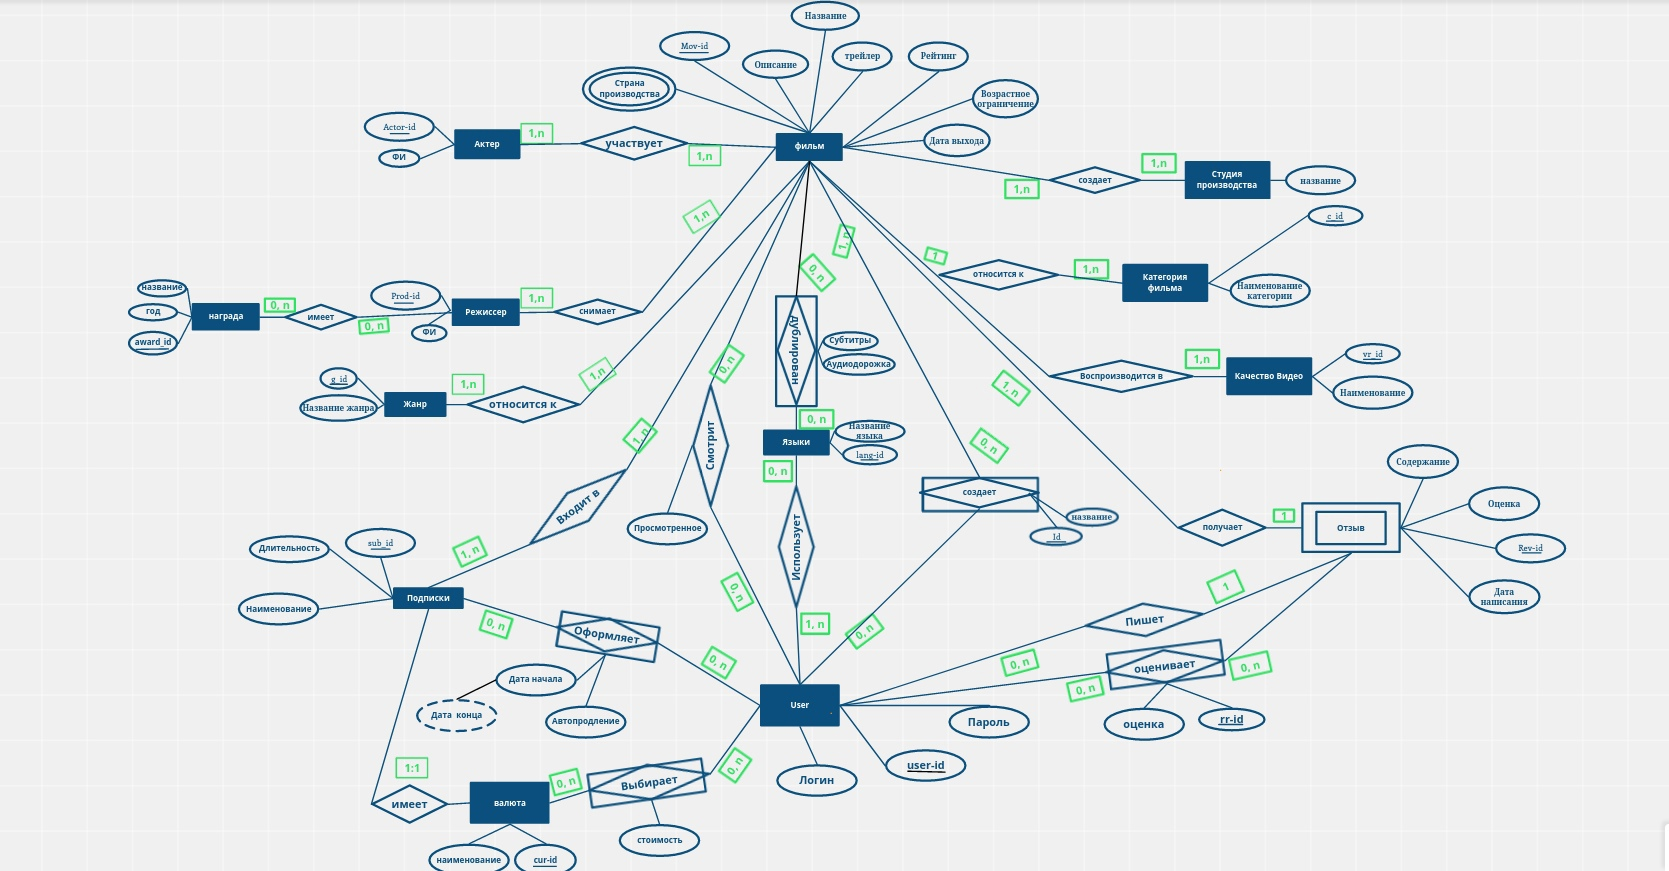
\includegraphics[width=1\linewidth]{concept}}
    \caption{Концептуальная модель базы данных}
\end{figure}

\subsection{Описание неочевидных атрибутов}
В процессе проектирования у сущностей были выделены следующие атрибуты:

\begin{enumerate}
\item Уникальные идентификаторы для каждой сущности: mov\_id, actor\_id (позднее act\_id), user\_id, award\_id,
cur\_id, sub\_id, rev\_id, prod\_id, lang\_id, watch\_id, g\_id, pc\_id, vr\_id
\item Наименование категории фильма -- его характеристика по хронометражу, то есть сериал, полнометражный, короткометражный и др.
\item Страна производства -- страна, в которой был снят фильм. Поскольку их может быть много, атрибут многозначный
\item Наименование качества видео -- разрешение в котором его можно смотреть.
\item Аудиодорожка и субтитры фильма -- разделены, поскольку пользователь может смотреть фильм, например, в оргинальной озвучке,
    но в субтитрах родного языка.
\end{enumerate}

\section{Логическое проектирование}
После завершения проектирования концептуальной модели базы данных, на ее основе была создана логическая модель,
представленная ниже:

\begin{figure} [H]
    \begin{subfigure}{.4\linewidth}
    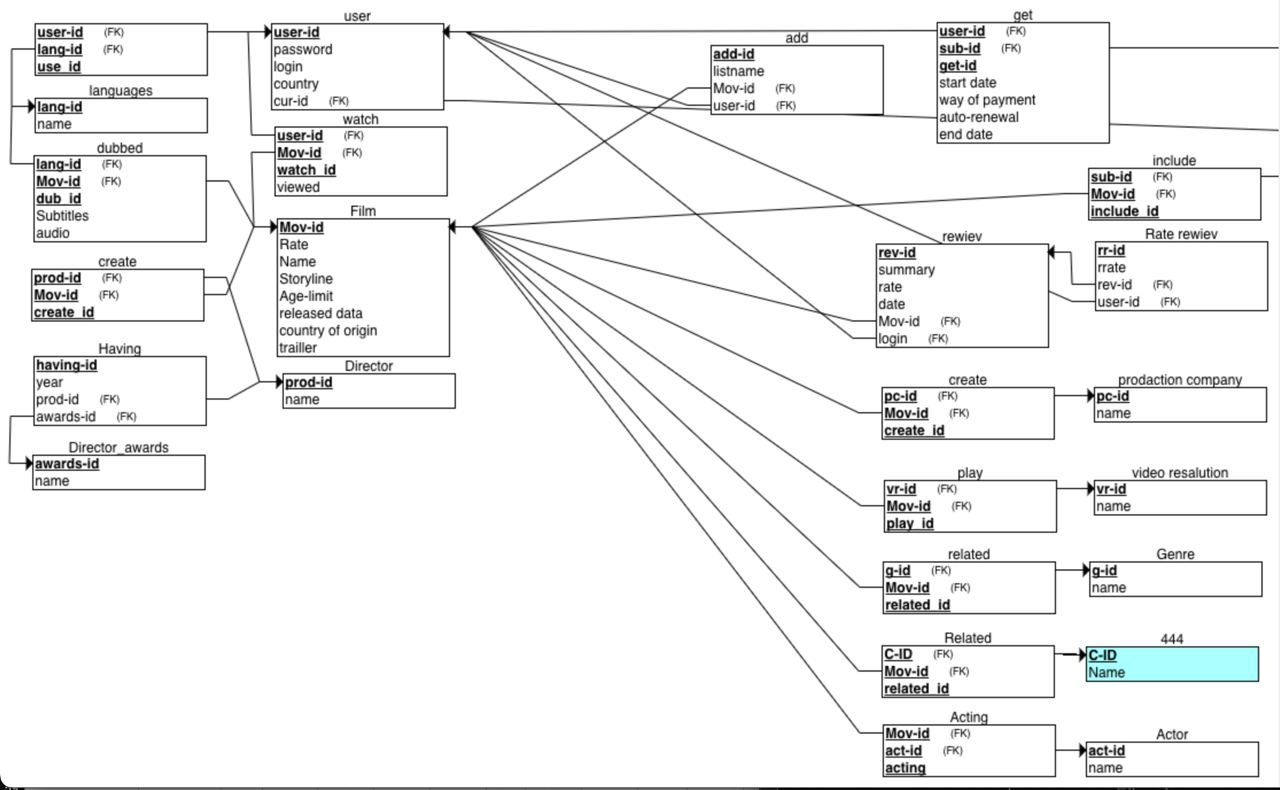
\includegraphics[width=2.6\linewidth]{logic1}
    \end{subfigure}

    \begin{subfigure}{.5\linewidth}
    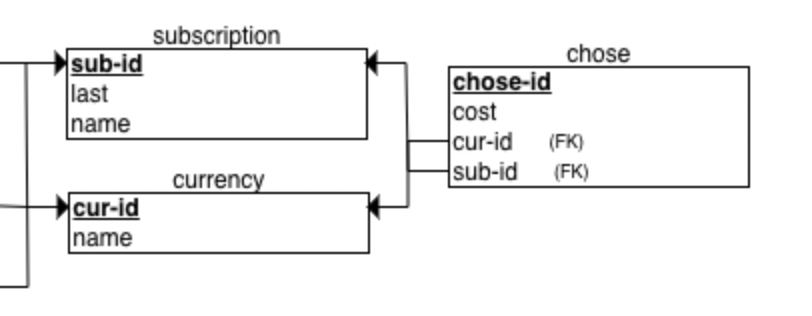
\includegraphics[width=1.5\linewidth]{logic2}
    \end{subfigure}

    \caption{Логическая модель базы данных}
    \label{logic}
\end{figure}

Все связи типа «Многие ко многим» были реализованы через отдельные таблицы.
\newpage

\section{Физическое проектирование}
В качестве СУБД для реализации разработанной базы данных была выбрана
PostgreSQL. Код для реализации таблиц основных сущностей представлен ниже:

Для таблицы Actor:
\begin{figure} [h!]
    \center{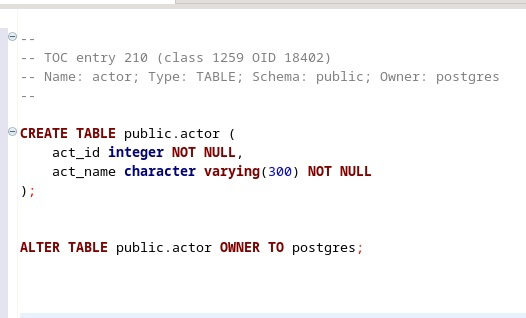
\includegraphics[width=0.8\linewidth]{actor}}
    \caption{Фрагмент кода для таблицы Actor}
\end{figure}

Для таблицы Film:
\begin{figure} [H]
    \center{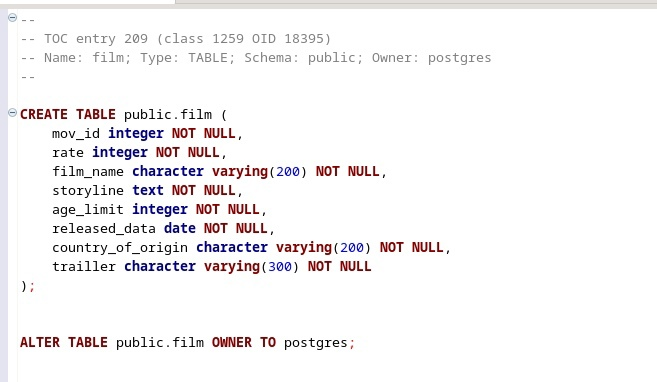
\includegraphics[width=0.8\linewidth]{film}}
    \caption{Фрагмент кода для таблицы Film}
    \label{film}
\end{figure}

Для таблицы User:
\begin{figure} [H]
    \center{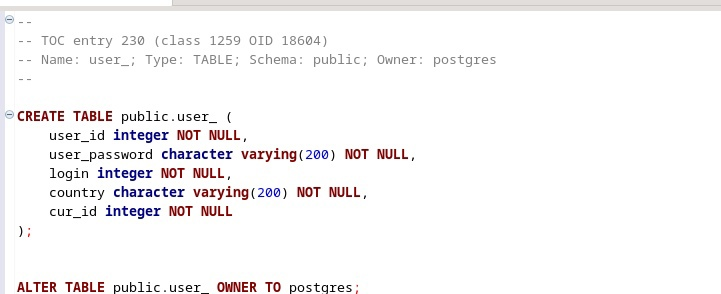
\includegraphics[width=0.8\linewidth]{user}}
    \caption{Фрагмент кода для таблицы User}
\end{figure}

Для таблицы Director:
\begin{figure} [H]
    \center{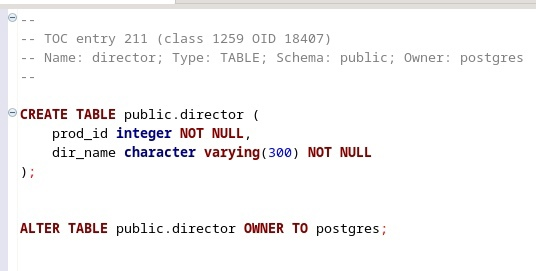
\includegraphics[width=0.8\linewidth]{director}}
    \caption{Фрагмент кода для таблицы Director}
\end{figure}

Для таблицы Awards:
\begin{figure} [H]
    \center{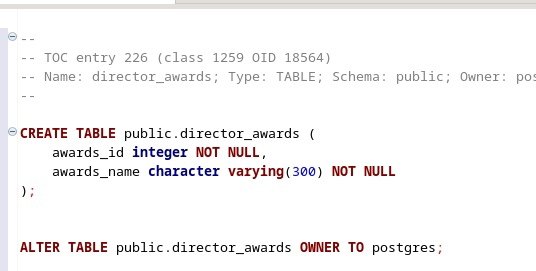
\includegraphics[width=0.8\linewidth]{awards}}
    \caption{Фрагмент кода для таблицы Awards}
\end{figure}

Для таблицы Genre:
\begin{figure} [H]
    \center{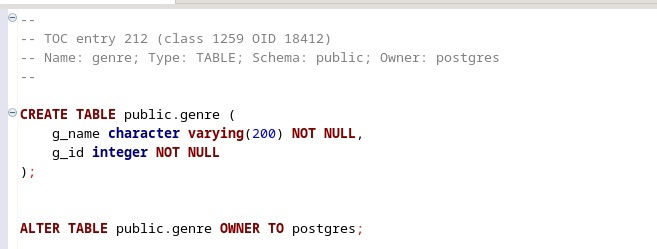
\includegraphics[width=0.8\linewidth]{genre}}
    \caption{Фрагмент кода для таблицы Genre}
\end{figure}

Для таблицы Review:
\begin{figure} [H]
    \center{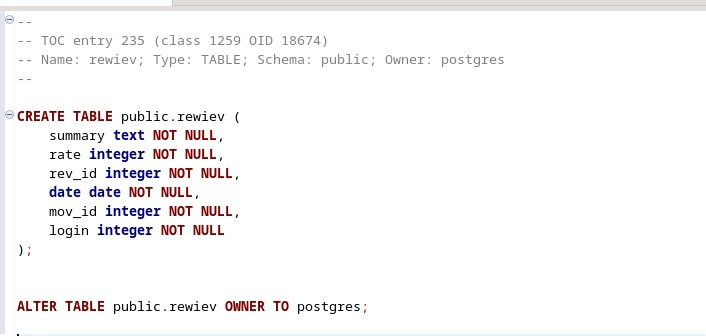
\includegraphics[width=0.8\linewidth]{review}}
    \caption{Фрагмент кода для таблицы Review}
\end{figure}

Для таблицы Languages:
\begin{figure} [H]
    \center{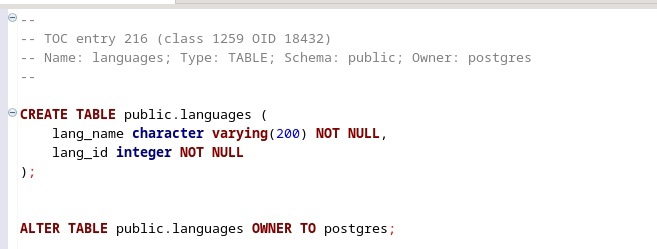
\includegraphics[width=0.8\linewidth]{langs}}
    \caption{Фрагмент кода для таблицы Languages}
\end{figure}

Для таблицы Category(хронометраж):
\begin{figure} [H]
    \center{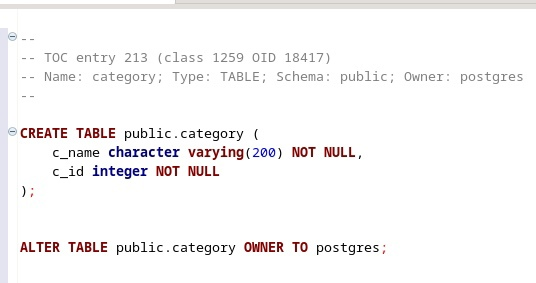
\includegraphics[width=0.8\linewidth]{category}}
    \caption{Фрагмент кода для таблицы Category}
\end{figure}

Для таблицы Rate review(оценок отзывов):
\begin{figure} [H]
    \center{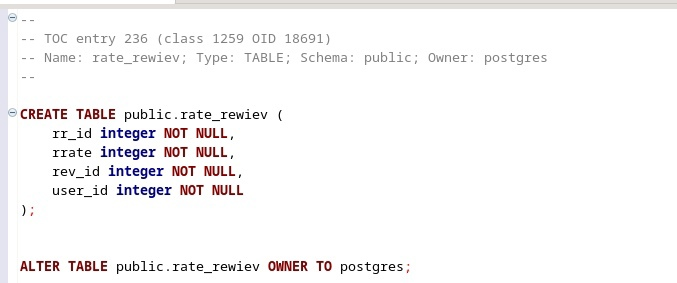
\includegraphics[width=0.8\linewidth]{rate_review}}
    \caption{Фрагмент кода для таблицы Rate review}
\end{figure}

Для таблицы Subtitles:
\begin{figure} [H]
    \center{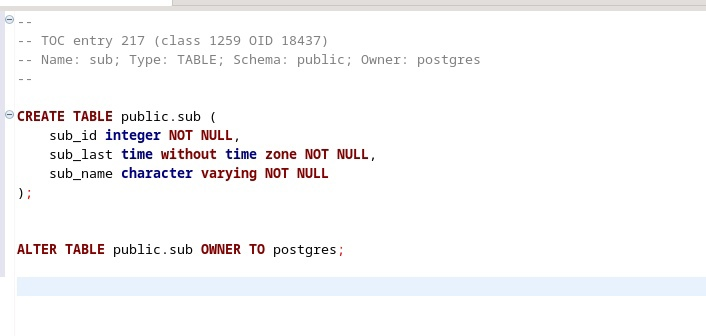
\includegraphics[width=0.8\linewidth]{subs}}
    \caption{Фрагмент кода для таблицы Subtitles}
\end{figure}

 Для таблицы Prodaction company:
\begin{figure} [H]
    \center{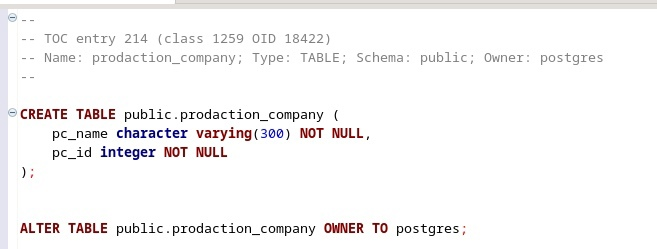
\includegraphics[width=0.8\linewidth]{prod_comp}}
    \caption{Фрагмент кода для таблицы Prodaction}
\end{figure}

\section{Заполнение данными}
Для заполнения данными использовался язык Python, а так же несколько инструментов. В общем и целом процесс
включал три стадии:

\begin{enumerate}
\item Написание python кода для заполнения таблиц случайными или не очень данными.
\item Перевод сгенерированных таблиц в csv формат
\item Собрание всех csv файлов и генерация единого SQL скрипта для заполнения базы данных.
\end{enumerate}

Следует отметить, что не все таблицы заполнялись рандомными данными. В частности, таблицы Films и
Review заполнялись исходя из датасетов с сайта kaggle 
\begin{itemize}
\item \url{https://www.kaggle.com/datasets/rounakbanik/the-movies-dataset},
\item \url{https://www.kaggle.com/datasets/lakshmi25npathi/imdb-dataset-of-50k-movie-reviews}
\end{itemize}

Фрагмент одного такого заполнения представлен ниже:

\begin{figure} [H]
    \center{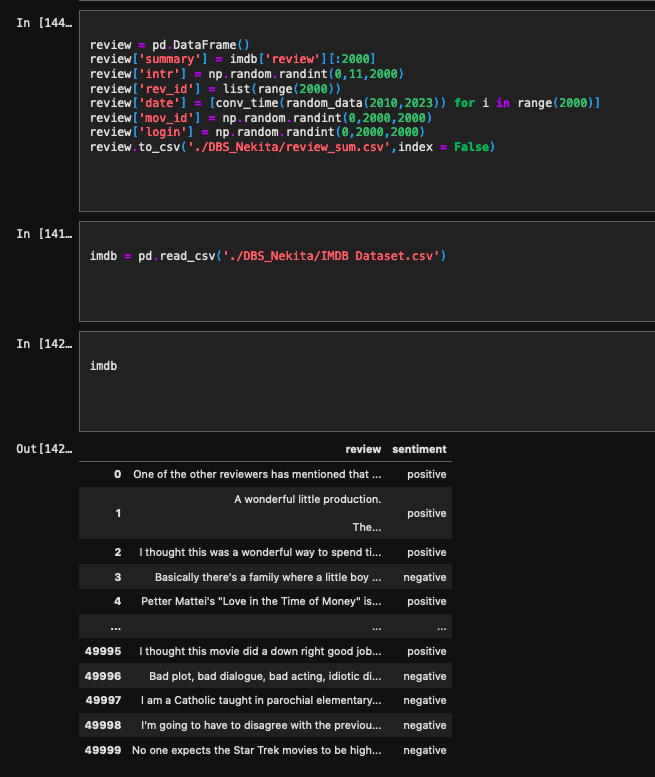
\includegraphics[width=0.8\linewidth]{IMDB}}
    \caption{Фрагмент кода для заполнения отзывов}
\end{figure}

Те же таблицы, которые заполнялись полностью случайными данными, потом переводились в csv формат
(например для таблица связи между просмотренным и режиссером):
\begin{figure} [H]
    \center{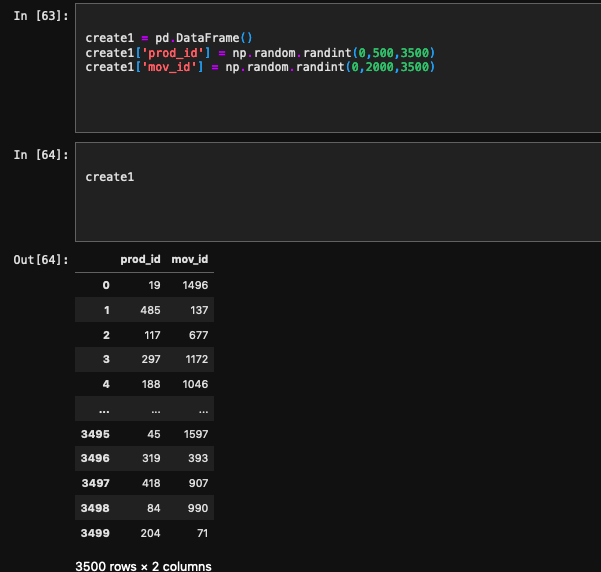
\includegraphics[width=0.8\linewidth]{rand}}
    \caption{Фрагмент кода для заполнения таблицы связи между просмотренным и режиссером}
\end{figure}

Для перевода данных в SQL скрипт для заполнения базы данных использовался сайт \url{https://konbert.com/convert/csv/to/sql}.

После генерации скрипта и его запуска, можно просмотреть содержимое некоторых таблиц:

Пример заполненной таблицы с данными об актерах:
\begin{figure} [H]
    \center{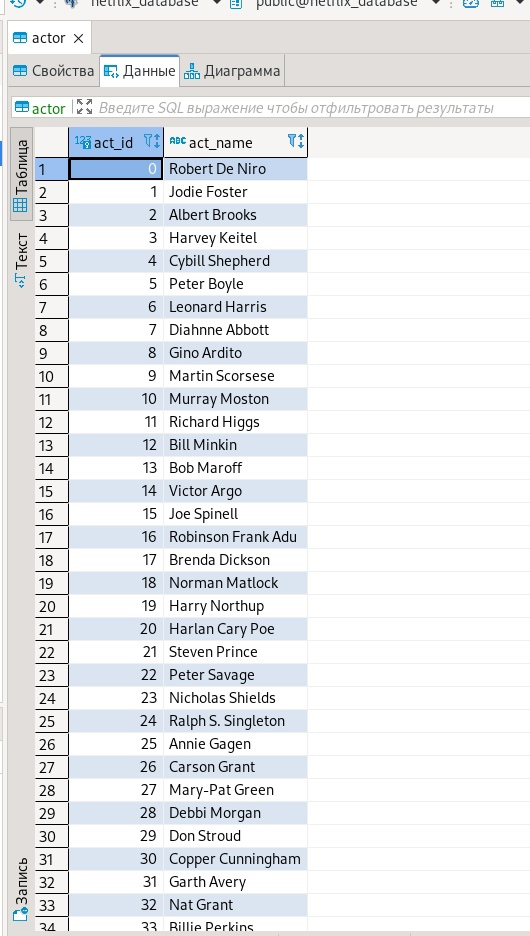
\includegraphics[width=0.8\linewidth]{ex1}}
    \caption{Заполненная таблица с именами актеров}
\end{figure}

Пример заполненной таблицы с данными о жанрах фильмов:
\begin{figure} [H]
    \center{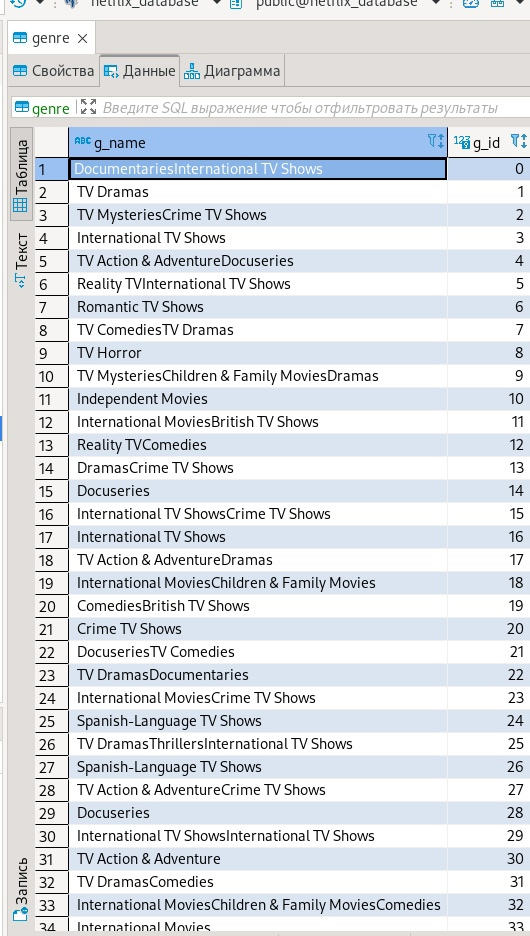
\includegraphics[width=0.8\linewidth]{genres}}
    \caption{Заполненная таблица с именами актеров}
\end{figure}

Пример заполненной таблицы с данными о названиях фильмов
\begin{figure}
    \center{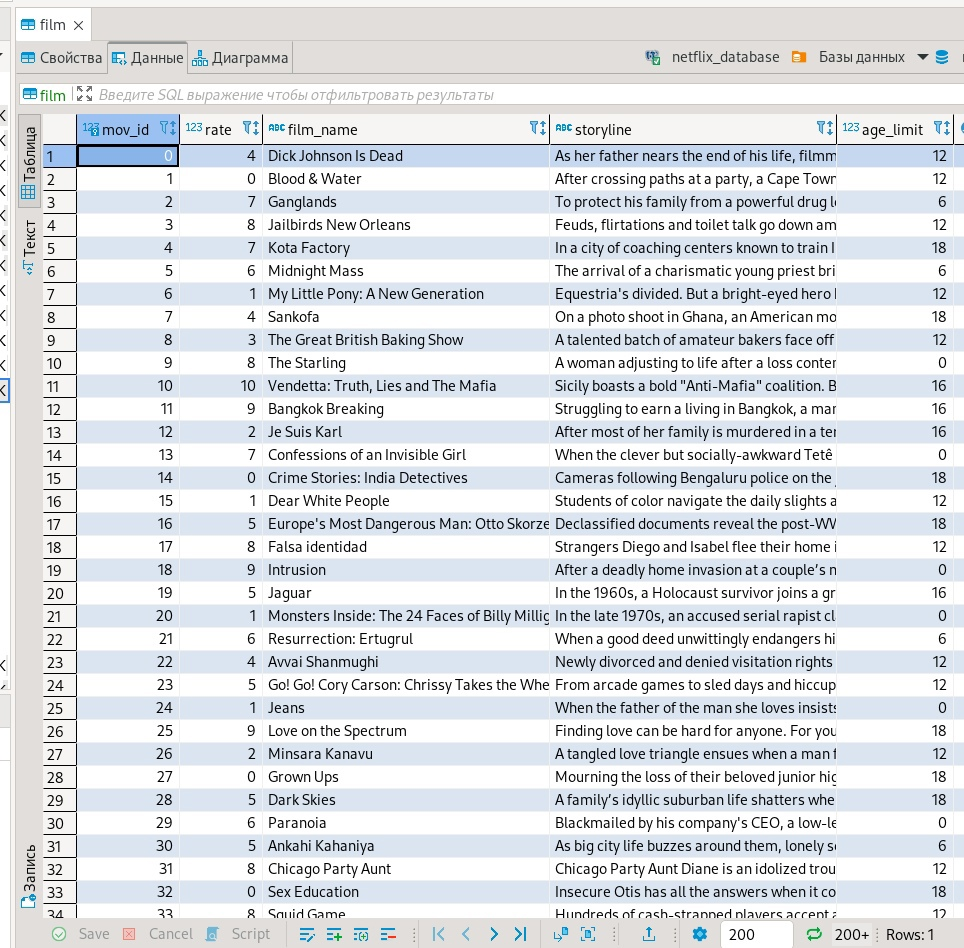
\includegraphics[width=0.9\linewidth]{names}}
    \caption{Заполненная таблица с названиями фильмов}
\end{figure}

\section{Реализация запросов}
Запросы писались к базе данных, сделанной по варианту "auto.ru". Содержание их следующее:
\begin{enumerate}
\item Вывести 5 самых старых пользователей с именем «Глеб»
\item Вывести id 10 самых быстрых машин с цветом "phantom black"
\item Вывести количество марок автомобилей, у которых разность между 
автомобилем имеющим максимальный пробег и минимальный пробег, среди всех 
моделей конкретно взятой марки не превосходило бы 50000.
\item Среди пользователей, которые отправили наибольшее количество сообщений, 
выбрать самого младшего и для него вывести разность между самым старым и самым 
новым выставленным им автомобилем.
\item Вывести среднюю цену для автомобилей с бензиновым двигателем и объемом от 2 до 4 литров c разгоном до 6 секунд.
\end{enumerate}


\end{document}
